\section{논문 요약}{\label{sec:review}}

\subsection{Multi-modal fusion transformer for end-to-end autonomous driving}{\label{subsec:Transfuser}}
\begin{figure}[htp]
    \centering
    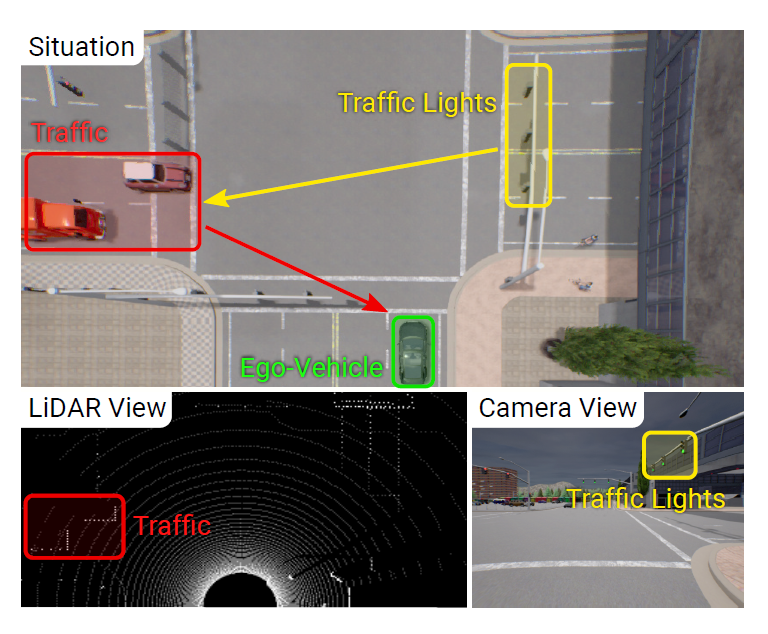
\includegraphics[width=0.8\textwidth]{figures/Transfuser_case.png}
    \caption{논문에서 해결하려는 문제 상황}
    \label{fig:tf_case}
\end{figure}
이 논문은 \autoref{fig:tf_case} 의 상황처럼
라이다(LiDAR : Light Detection And Ranging) 센서로 얻을 수 있는 주변의 차량의 위치에 따른 교통정보와
카메라로 얻을 수 있는 신호기에 따른 교통정보가 다른 경우,
두 센서로부터 얻을 수 있는 정보를 결합하여 차량의 주행을 제어하는 것을 목적으로 한다.
\begin{figure}[htp]
    \centering
    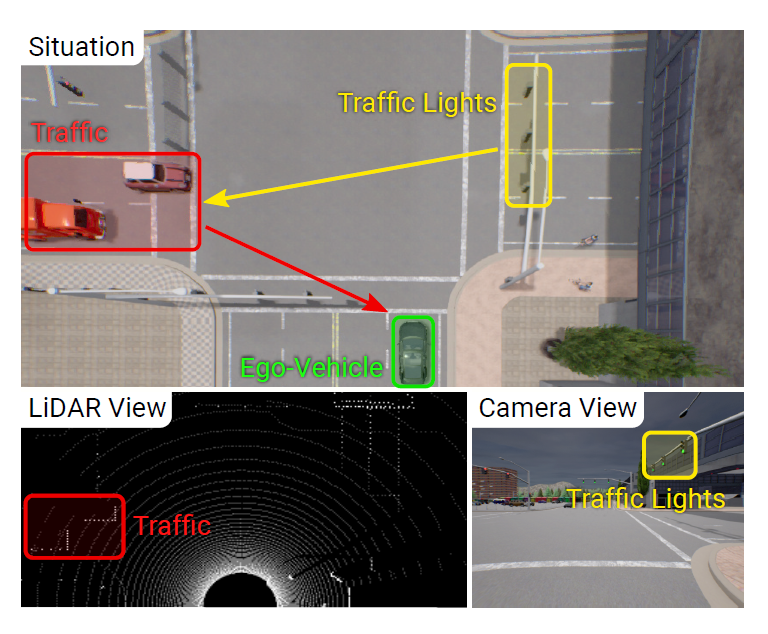
\includegraphics[width=\textwidth]{figures/Transfuser.png}
    \caption{Transfuser 구조}
    \label{fig:tf}
\end{figure}
\autoref{fig:tf}는 Transfuser의 구조를 보여준다.
두 센서의 출력으로부터 Resnet 구조\cite{Resnet}를 이용하여 정보를 추출하는 과정에서,
각 layer의 출력단으로부터 추출된 정보를 Transformer\cite{Transformer}를 이용하여 결합하는 것을 확인할 수 있다.


\subsection{YOLOv7: Trainable bag-of-freebies sets new state-of-the-art for real-time object detectors}{\label{subsec:yolov7}}

asdf